\chapter{Protein Location Relation Extraction: Materials \& Methods}\label{chapter:methods}
\newcommand*{\xml}[1]{\texttt{<#1>}}
\section{Task Definition}

%TODO Refer to the actual section of relatione extraction
This chapter explains the method developed to extract protein-location relations from biomedical text. This task of relation extraction comes under the broad category of natural language processing (NLP) as explained in the section \ref{sec:RE}. The task of extraction of Protein-Location relations can be formally described as follows:

Given a piece of text that contains two entity mentions, viz. protein and location, the task of relation extraction method is to decide if the text contains enough evidence for semantic relationship between these two entities. Formally, let $r=(t,arg_1,arg_2)$ denote a relationship instance where $t$ is a piece of text, $arg_1$ and $arg_2$  are entity mentions contained in text $t$, and $arg_1$ precedes $arg_2$ in the text. Given a set of relations $\left\lbrace r_i \right\rbrace$ such that every relation instance has label $l \in \left\lbrace-1,1\right\rbrace$, our task is to learn a function that can predict the label $l$ for new relation instance whose label is not known. Note that $t$ can simply be a piece of text or it may also contain structured information such as parse tree and dependency graphs. For entity mentions $arg_1$ and $arg_2$, either of them can represent a protein or a location entity.
 
% Following section to be deleted, to be shifted to introduction
\section{Replication of the state of the art in BioNLP'09}

% where should I put that
Section \ref{sec:JariBioNLP} describes the method developed by Björne et al. for the task of event extraction in BioNLP 2009. The method developed by Björne et al. along with several other methods for various tasks is available online at \url{http://jbjorne.github.io/TEES/}. I used the package TEES (Turku Event Extraction System) to get started and tried to replicate the results of his model for the task of event extraction. The selection of features in my model is influenced by the features used for the task of event extraction in TEES.

%\section{Method for protein-location relation extraction}
\subsection*{Outline of the chapter}

I will describe the method that I developed for the extraction of protein-location relations in subsequent sections. Here is the overview of sections in this chapter: 

Section \ref{sec:ssModeldsModel} explains the motivation for creating more than 1 machine learning model. Section \ref{sec:pipeline} outlines the flow of information in this task of relation extraction. Section \ref{sec:models} introduces the machine learning models. Section \ref{sec:graphRep} explains the actual representation of data in the model. The process of feature extraction and feature selection is explained in section \ref{sec:featExp} and \ref{sec:featSel} respectively.

The training methodologies and procedures are explained in section \ref{sec:training}. Section \ref{sec:experiments} talks about all different experiments tried and their effect on the overall method. Finally, section \ref{sec:tools} concludes with describing the tools used in the task.

\section{Motivation for creating multiple machine learning models}\label{sec:ssModeldsModel}

The protein-location relation is a semantic relation between a protein entity and a location entity present in the text. As explained in the section \ref{sec:corpusStats}, the protein-location relations are categorized into two key categories, viz. same sentence relations and different sentence relations. Same sentence relations are the relations in which both protein and location entity are present in the same sentence. Different sentence relations are the ones in which either of the participating entities lie in different sentence.

As discussed in the section \ref{sec:corpusStats}, around 63.81\% of total protein-location relations are same sentence relations while the remaining 36.19\% are different sentence relations. A sentence can be considered as a unit of text where grammatical rules are strictly followed. The rules that define the relationship between entities in the same sentence can be different from the rules that define the relationship between entities in the different sentence. In other words, the feature set for extracting same sentence relations could be different from the one used for extracting different sentence relations. Combining both feature sets can possibly decrease the performance of both the tasks, viz. same sentence protein-location relation extraction and different sentence protein-location relation extraction. Therefore, I decided to develop two machine learning models, one of which would be dedicated to extracting same sentence relations and the other one would be dedicated for extracting different sentence relations.

Furthermore, the semantic relationship between protein and location in the case of different sentence relations with large sentence distances might be difficult to extract due to intermittent noise and hence, I tried to focus only on those different sentence relations which have a sentence distance of 1, i.e., the protein and location entities are found in neighboring sentence.

The same sentence model designed for extracting same sentence relations would be  abbreviated as \textit{SSModel} hereafter for the purpose of brevity. The different sentence model designed for extracting different sentence relations would be abbreviated as \textit{DSModel} for the same purpose.

\section{Graph representation} \label{sec:graphRep}
% Details about graph representation along with nice explanatory picture

\subsection{Graph representation for \textit{SSModel}}\label{sec:graphSSModel}

\subsection{Graph representation for \textit{DSModel}}\label{sec:graphDSModel}


\section{Method pipeline}\label{sec:pipeline}

%- Explain the whole pipeline 
%- Corpus-->Sentence Segmentation-->Tokenization-->Syntactic & dependency Parsing-->Graph Representation-->  Feature Extraction --> ML Model training -->Classification on Test
%- Put a nice picture explaining the pipeline

The overall relation extraction method consists of following major stages:

\begin{enumerate}

\item \textbf{Data collection \& Corpus creation}

For LocText corpus, the annotated data is present in the JSON files that can be downloaded through the tagtog web-interface \cite{cejuela2014tagtog}. However, the JSON files only contains the text of the annotations. The whole document text is present in a separate set of HTML files. Every JSON or HTML file corresponds to particular MEDLINE \cite{medline} document. To avoid reading from plain files repeatedly, I decided to create a XML file containing all the corpus data along with annotations and structural details like parse tree, dependency graphs etc.

\begin{figure}
\centering
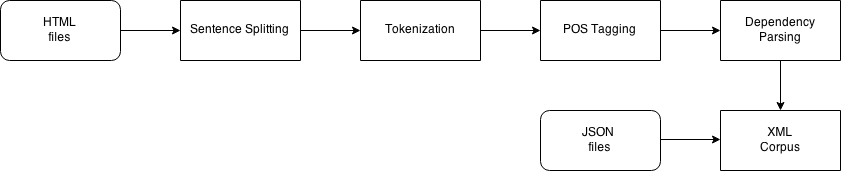
\includegraphics[scale=0.4]{figures/Corpus_Creation.png}
\caption{The process of creating a XML corpus file}\label{fig:corpusCreation}
\end{figure}

Figure \ref{fig:corpusCreation} outlines the process  of corpus creation. The data read from HTML files is parsed using Stanford CoreNLP pipeline \cite{manning2014stanford}. In every HTML file, the data is divided into title and abstract. The text from HTML files which consists of title and abstract is initially segmented into sentences (\textit{Sentence Splitting}). Every sentences is then split into tokens (\textit{Tokenization}). Part of the speech tags are found out for every token (\textit{POS Tagging}). Finally, the dependency relations between the tokens in the sentence are computed (\textit{Dependency Parsing}). These stages of processing are explained in detail in the section \ref{sec:NLPPipeline}.

All the unstructured (plain text) and structured (sentences, tokens, POS tags, dependencies) information is then combined with annotations present in JSON files and written to the XML corpus file.

\begin{figure}
\centering
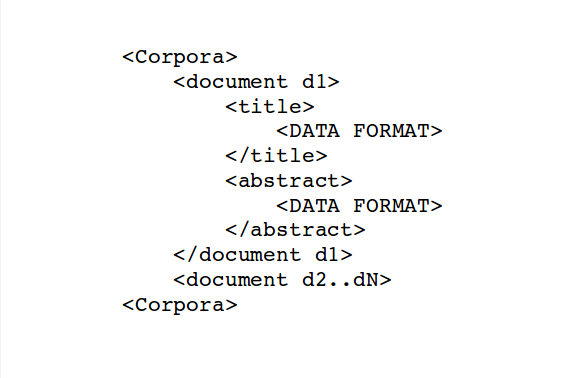
\includegraphics[scale=0.4]{figures/XMLSchema1.png}
\caption{Coarse XML schema}\label{fig:XMLSchema1}
\end{figure}

The coarse XML schema of the corpus XML file can be shown in the fig. \ref{fig:XMLSchema1}. Every document (corresponds to a MEDLINE document) has two sections, viz. title and abstract. Both sections have similar structure of internal data representation denoted by "DATA FORMAT". The data representation format "DATA FORMAT" is elaborated in fig. \ref{fig:XMLSchema2}.

\begin{figure}
\centering
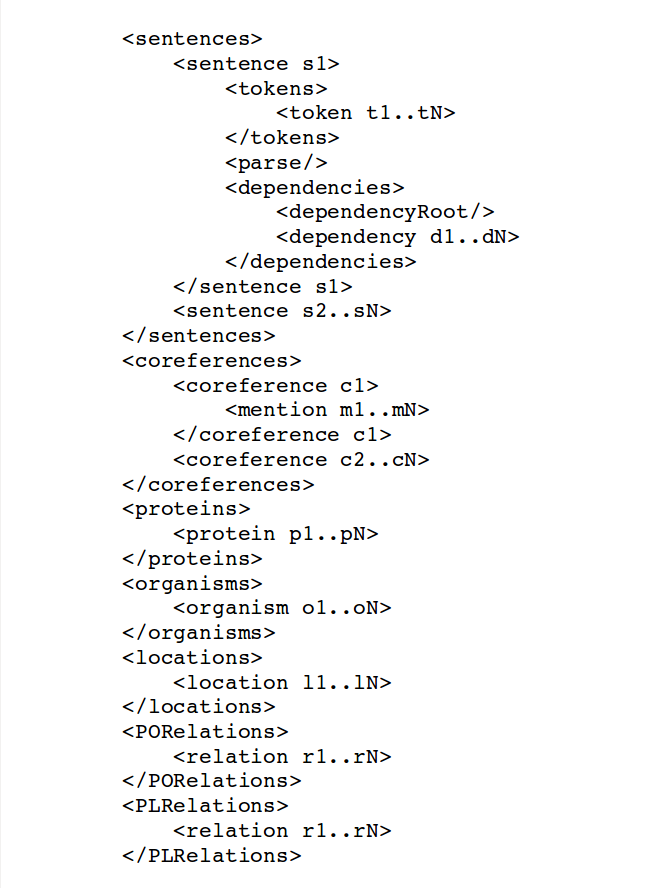
\includegraphics[scale=0.4]{figures/XMLSchema2.png}
\caption{Data format common to title and abstract node}\label{fig:XMLSchema2}
\end{figure}

The "DATA FORMAT" shown in fig. \ref{fig:XMLSchema2} represents the XML format used to store the data inside the title and abstract node. The nested nodes are displayed with a tab indentation. The figure is representative and does not repeat the structures of nodes for similar parent nodes. For example, even though only the node \texttt{sentence s1} shows the structure of internal nodes like tokens, essentially all the sentence nodes \texttt{sentence s2..sN} have same structure of the internal nodes.

The nodes in the "DATA FORMAT" can be explained as follows:

\begin{itemize}
\item \texttt{sentences}: This node represents collection of sentences.
  \begin{itemize}
  \item \texttt{sentence}: a basic sentence unit, containing information such as sentence text, start offset, end offset, etc.
    \begin{itemize}
	\item \texttt{tokens}: collection of tokens
	  \begin{itemize}	  
	  \item \texttt{token}	: a basic token unit containing information such as text of token, starting offset, end offset, POS tag, etc.		
	  \end{itemize}
	\item \texttt{parse}: a syntactic parse tree of the sentence
	\item \texttt{dependencies}: collection of dependencies between the tokens	  
	  \begin{itemize}
	  \item \texttt{dependency}: a dependency relation containing information such as from token, to token, dependency type, etc.
	  \end{itemize}	  
	\end{itemize}	
  \end{itemize}
  \item \texttt{coreferences}:
    This node is a collection of coreferences present in the entire text unit (title or abstract)
    \begin{itemize}
    \item \texttt{coreference}: a collection of coreferent mentions
    \begin{itemize}
      \item \texttt{mention}: it contains information about text of the coreferent mention, start token in the sentence, end token and whether this is a representative mention or not.
    \end{itemize}
    \end{itemize}

\item \texttt{proteins}: protein entity annotations
\item \texttt{organisms}: organism entity annotations
\item \texttt{locations}: subcellular location entity annotations
\item \texttt{PORelations}: protein-organism relation annotations
\item \texttt{PLRelations}: protein-location relation annotations
\end{itemize}

\item \textbf{Training \& evaluating \textit{SSModel}}

This is the second step in relation extraction method. This step focuses solely on extracting same sentence protein-location relations from the text. The data is read from the corpus XML file. 

Every document is processed one by one. From every documents, the sentences and the allied information is loaded into data strucutres.

\item \textbf{Training \& evaluating different sentence model}

\item \textbf{Combined evaluation}

\end{enumerate}

\section{Machine Learning Models}\label{sec:models}
% Talk about different models here so that there is no confusion ahead

\subsection{SameSentenceModel}

\subsection{DiffSentenceModel}


\section{Feature extraction}\label{sec:featExp}

\subsection{Feature extraction for SameSentenceModel}

\subsection{Feature extraction for DiffSentenceModel}

\section{Feature Selection}\label{sec:featSel}

%Write some of the results found out from in Joachim's paper [Text categorization with SVM]
%
%**This is a very important property that has got to be known that in text categorization using SVM, there are only few irrelevant features.
%
%When ranked according to Binary information gain, see Figure 1, removal of high ranking features does not take away a lot of information. This also means that even features ranked lowest still contain considerable information and are somewhat relevant.
%
%TODO: See how to calculate binary information gain for a feature/set of features.***

\section{Training, Cross validation and Classification}\label{sec:training}

\section{Experiments that worked and that did not work}\label{sec:experiments}

\subsection{Experimentation for SameSentModel}

- Removing sentences which had no proteins improved the performance
- Using different kernels did not work

\subsection{Experimentation for DiffSentModel}

- Using extra information from the document such as shortform longform pairs decreased the performance since it added more FP's (15) than TP's (1). It seems that this rule was nicely followed during annotation

\subsection{Experimentation with different kernels}

\section{Tools used}\label{sec:tools}
